\section{Employment of AWS EC2}
As mentioned in the previous chapter, the full flexibility is available, which means full access to the operation system is available and there can be installed and used almost every software if desired. Therefore the disadvantage of the comprehensive flexibility is, to manage the whole system and software by everyone itself. There exists no automatic measurements or load balancing systems provided by the IaaS provider, it has to be implemented a load distribution system by itself. 

In further steps it has to be defined, what is the reaction if one server cannot handle anymore the work which is intended for a particular server. There has to be an ongoing monitoring in place which checks various key indicators regularly and reports its measurements back to a central system which therefore decides if more or less servers are necessary than currently used.

%The most important indicators for an overloaded system is a too high cpu utilisation. But also the memory consumption as well as network traffic, number of request or I/O load, may slow down the work of a server. Furthermore Unix and Linux systems report the system load .... (Thomas Bachelooooaaaaar Arbeit)
% What is load?


\subsection{Workload distribution}
In the case of the tweet classification the focus of the decision algorithm has to lie on the cpu utilisation, because the bottleneck of the classification algorithm is the available CPU. But just using the current CPU utilisation of each instance as a decision basis for request distribution seems too easy. Every time a particular instance receives a new request, the CPU utilisation raises up very quickly to about 100~percent and after finishing the tweet classification it gets back to idling. The distribution algorithm may forward request to an instance only if it is in idling state. Decisions based on this mercurial indicator may result in a system which waits to finish for classification until new requests are forwarded to an instance. This behaviour results to instances which are idling sometimes and are just waiting for new requests, also when the overall system is under heavy load. 

The algorithm may be improved if it assumes that each classification request fully utilises the CPU on the instance for a specific amount of time. After finishing the classification the utilisation goes down and a new request can be classified. The efficiency of the overall system can be improved if each instance is responsible for two requests at a time. The instance can immediately switch over to the second request after the first classification is finished. 

This consideration results in the decision algorithm that requests are forwarded to instances depending on the currently executed classification of each instance. Instances with no classification job right now should be preferred when distributing a new request. Those instances are idling and wasting money. If there are no idling instances available new classification jobs should be processed by instances which have just one classification running right now. They may will finished their currently running classification very soon and may drop back to idling if they don't receive a new request. But there should be no more than two classifications distributed to a particular instance at a time. This only results in longer time for finishing the classifications. To come up with short request peaks it may be necessary to forward more than two requests to a particular instance at a time. Instances with less concurrent requests should be always preferred. If instances receive more than two requests at a time for a longer period of time it is necessary to start new instances.


\subsection{Decision to start and stop instances}
As described in the previous section no instance should be responsible for more than two requests at a time. If there is a need to distribute three requests to at least one instance at a time it may indicates that the current amount of instances are not sufficient anymore to come by with the current request rate.

It looks obvious to start new instances if the requests increases the two-for-each-instance rate and stop an instance if it is idling. But this approach only works quite well if instances can be started immediately and are accounted per second. Unfortunately, both assumptions are not the case. Instances needs to start up to a couple of minutes and are accounted on an hourly basis. In conclusion there is a need for a different decision algorithm to start and stop instances. 

As stated by \citet{walker2006} Unix and Linux systems report values, the so-called load average. This load average reports the number of processes which demands for the CPU. Due to not only provide and instantaneous snapshot the actual CPU utilisation the load average gives a trend of the prospective CPU requirement. This computation consists of three values, the 1-minute, 5-minute and 15-minute load average. 

The load average value reports the number 0.00 for an idling system and 1.00 for a busy system. There are no limits for this numbers, but a load of 1.00 can be assumed as busy for the system. 

To employ the load average value for the decision algorithm it has to be clearly defined when the overall system needs more or less instances than currently started. The load of the overall system can be calculated by the average of the load of each instance. As already mentioned a load of 1.00 indicates that a system is busy, therefore this number should be avoided for the overall system. As \citet{brebner} suggests, it seems quite ok to start new instances if the overall system reaches the load of 0.8. In contrast to stop instances the load should be decreased quite more than to 0.8 to overcome fluctuation request rates and therefore load averages. Furthermore the stop of an instance should be as lazy as necessary to avoid the need to start a new instance quite short after the stop. It's necessary for future research about the best value, but for now the results of \citet{brebner} are considered, therefore instances will be stopped at the load of the overall system of 0.3. 

Furthermore there are three values of the load average reported, one for the 1-minute, 5-minute and 15-minute time period. To add some additional laziness to the decision algorithm not the most fluctuating value, the 1-minute load average, is chosen, but the 5-minute load average. However some additional research in place is required to verify this decision.  

In further consideration it may happen that there is a need for starting or stopping more than just one instance at a time. If there is a very fast increasing request rate there may be a need to start two or more instances simultaneously. To come by to this problem a simple load forecast can be employed. Each starting instance can be added to the load average with a load of 0.00 because this value is read quite short after the instance is ready for processing requests. If the load with this forecasted value in place is still more than the limit of 0.9 it is necessary to start additional instances. 

A quite similar assumption can be done for stopping instances, but there is a load of 1.0 assumed for every stopping instance. This forecast meets the issue that as soon as the instance is stopped the load of the overall system increases again beyond its limit and a new instance is started quite short after another instance was stopped.

%
%\subsection{Load Measurement}
%To find the actual key parameters when a particular server cannot serve anymore the work which is intended to do, it has to find out the bottlenecks. There exists no general measurement for every conceivable application to decide whether the application overloads the server or not. In the our case, the classification of the sentimental analysis of tweets the CPU is the bottleneck. The memory or network are not that hardly used as the CPU. Therefore it can be measured the load which is reported by Linux to decide whether the server runs out of resources or is in idling.
%
%The load value fits good for applications which have a very high CPU consumption, but have no or small external dependencies. There exists scenarios where a server may get a very high load value, but have no troubles at all. If an external database takes very long to answer the requests the server indicates a very high load value, but the assumption of an overloaded server is wrong.
%
%%Gedanken zur Auslastung: 
%%\begin{itemize}
%%\item CPU
%%\item Memory
%%\item Request/Sec
%%\item Anzahl gleichzeitiger Requests
%%\item Load
%%\end{itemize}
%
%\subsection{Load/Request/Work Distribution}
%There exists several algorithms to distribute a given amount of workload to various servers. The most common are Round-Robin or Random algorithms. But they do not respect the current utilisation of the servers. The one fits best for this project is the State algorithm. Each server enters the state "accept" on startup and is able to receive new connections. Once the server reaches a load value of 0.7 the state changes to "reject" and there can not be new requests until the server load decreases back to 0.7 or less and the server gets back to it's initial state.
%
%\begin{figure}[H]
%  \centering
%  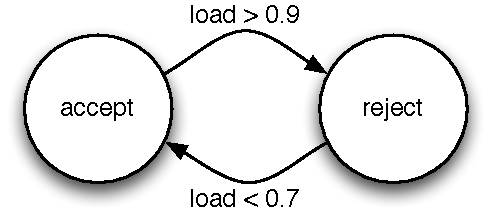
\includegraphics[width=0.85\linewidth]{images/state.pdf}
%  \caption{State Diagram}
%  \label{fig:state}
%\end{figure}
%
%
%The actual load distribution is done by CloudScale. This library intercepts requests to particular methods and forwards them to an instance of the application which is executed on the cloud. Furthermore CloudScale asks the application to which node a method call should be forwarded. This method interception and forwarding is transparent to the caller.
%
%\subsection{Decision Criteria -  Nodes Start/Ende}
%In addition to the knowledge of the utilisation of each server there has to be decisions in place whether an application has to be deployed to more servers or if the application is currently deployed to more server than necessary. In best cases there should at no time more server utilised than actual needed, but neither less server than mandatory. The decision algorithm has also to regard that every running server generates costs and newly started server takes quite a while to finish booting. There are many more parameters which have to be considered, such as the expected load for the future.
%
%The load value computation can be extended to an computation for the whole cloud. The average value of all load values of all servers indicates the load of the whole cloud. An average load for the whole cloud of less than 0.7 seems quite ok, whereas the average reaches a value closer to 1 indicates that the cloud can not handle all requests as required. To overcome very high load values it makes sense to start new instances with respect to the load which can be forecasted after starting the instance. The load value for a newly started instance is 0 and this value can be very easily added to the average of load values for the whole cloud. If there are already many instances started, just 1 new started instance do not have much effect on the overall system and it may be needful to start more instances at once. 
%
%Also the decision on the shutdown of no longer needed instances can be done on the basis of the average load value. There can also be a forecast in place, which works quite the same as for starting new instances. To stopping instances should be a more longer-term decision than the algorithm which starts new server, because suddenly appearing request spikes have to be handled by new instances, whereas instances which are just idling do not harm the performance of the cloud. But with respect to the costs, instances which are no longer needed to come by to the load should be closed down.
%
%There exists a paper 

%\subsection{Entscheidung mit Puffer}


% Kommt zu paas: In contrast to the IaaS provider a PaaS provider still have the full control over the system and just executs your software on his cloud. The PaaS provider usually monitors his cloud and distributes your (and many more) application depending on the load of the application. You don't have to do anything if your application runs into high requests, the provider automaticlly distrributes your application without anything done by you, such as manual deployment to other servers or and implemented solution for automatic distribution. 